% !TEX program = xelatex

% Základní balíčky
\documentclass[10pt,a4paper]{article}
\usepackage[utf8]{inputenc}
\usepackage[T1]{fontenc}
\usepackage{graphicx}
\usepackage{wrapfig}
\usepackage{nonfloat}
\usepackage{amsmath}
\usepackage{amssymb}
\usepackage{mathtools}
\usepackage{hyperref}
\usepackage{gensymb}
\usepackage[top = 1cm, bottom = 1cm, left = 1cm, right = 1cm]{geometry}

% Language-related
\usepackage[czech]{babel}
\usepackage{csquotes}
\usepackage{polyglossia}
\setmainlanguage{czech}
\setotherlanguage{greek}

% Bibtex je oficiálně mrtka
% \usepackage[backend=bibtex,style=verbose-trad2]{biblatex}
% \usepackage{etoolbox}
% \patchcmd{\thebibliography}{\section*{\refname}}{}{}{}
% \bibliography{protokol}

% Pro titulní stránku
\usepackage{titlesec}
\usepackage{setspace}
\usepackage{framed}
\usepackage{array}

% Vlastní balíčky
\usepackage{gnuplottex}
\usepackage{epstopdf}
\usepackage{csvsimple}
\usepackage{units}
\usepackage{subfig}
\usepackage{pdfpages}
\usepackage{multirow}

\usepackage{soul}

\usepackage{calc}
\newcommand*{\mask}[2]{\mathord{\makebox[\widthof{\(#1\)}]{\(#2\)}}}




\renewcommand{\U}[1]{\ensuremath{\,\mathrm{#1}}}
\newcommand{\°}{\degree}

\newcommand{\titjmeno}{Michal Grňo}
\newcommand{\titobor}{FOF}


\newcommand{\titcislo}{A19}
\newcommand{\titnazev}{Rentgenografické difrakční určení mřížového parametru známé kubické látky}
\newcommand{\titmereni}{19. 11. 2020}
\newcommand{\titodevzdani}{4. 12. 2020}


\renewcommand{\t}[1]{\mathrm{#1}}


\begin{document}


\thispagestyle{empty}
\newgeometry{top = 2.5cm, bottom = 0cm, left = 2.5cm, right = 3cm}

{%T tomto je uzavřena celá titulka
%Tloušťka rámečku
\setlength{\fboxrule}{1.5pt}

\noindent
\framebox{
\begin{minipage}{\textwidth}
\setlength{\parindent}{17.62482 pt}
\phantom{d}

\begin{minipage}{0.6\textwidth}
{
\Large Kabinet výuky obecné fyziky, UK MFF\\
}
\vspace*{0.2cm}

{
\bfseries
\huge Fyzikální praktikum %ČÍSLO
}
\end{minipage}
\begin{minipage}{0.4\textwidth}
\begin{center}
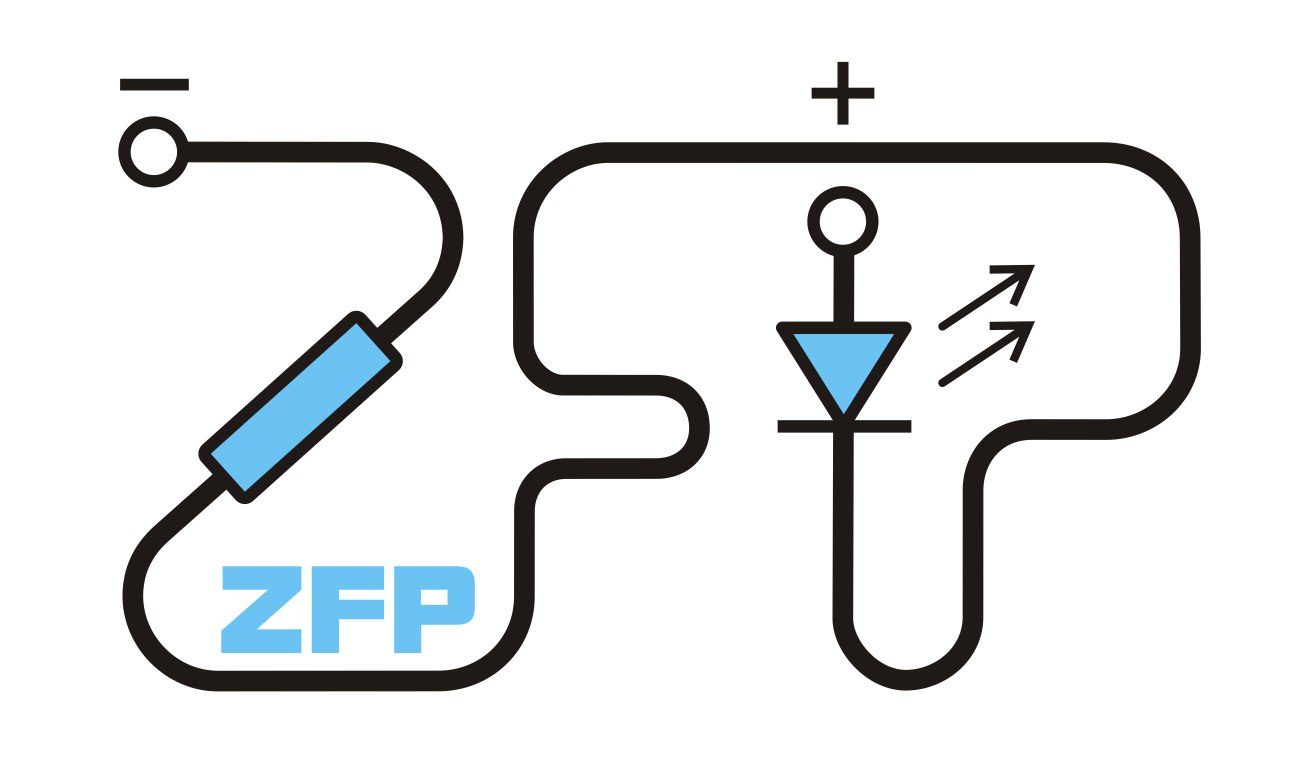
\includegraphics[width=4.5cm]{ZFP.jpg}
\end{center}
\end{minipage}\\\\

%\vspace*{0.5cm}

{
\setstretch{1.5}
\Large
\noindent
Úloha č. \titcislo

\noindent
Název úlohy: \titnazev

\noindent
Jméno: \titjmeno
\hspace*{\fill}
Obor: \titobor

\noindent
Datum měření: \titmereni
\hspace*{\fill}
Datum odevzdání: \titodevzdani

\phantom{d}
}
\end{minipage}
}
%Konec horního rámečku

{
\phantom{d}

\Large
Připomínky opravujícího:\\
\vspace*{6.75cm}
}

\newcommand{\linka}{\noalign{\hrule height 1pt}}
\newcommand{\linkadva}{\noalign{\hrule height 1.5pt}}
\setlength\extrarowheight{9.5pt}
\Large
\noindent
\begin{tabular}{!{\vrule width 1.5pt} l !{\vrule width 1pt} c !{\vrule width 1pt} c !{\vrule width 1.5pt}}
\linkadva
   & Možný počet bodů & Udělený počet bodů \\\linkadva
  Práce při měření & 0-3 &  \\\linka
  Teoretická část & 0-2 &  \\\linka
  Výsledky a zpracování měření & 0-9 &  \\\linka
  Diskuse výsledků & 0-4 &  \\\linka
  Závěr & 0-1 &  \\\linka
  Použitá literatura & 0-1 &  \\\linkadva
  \hspace*{\fill} \textbf{Celkem} \hspace*{\fill}& max. 20 &  \\
\linkadva
\end{tabular}
\phantom{d}

Posuzoval: \hspace*{\fill}dne:~~~~~~~~~~~~~~~~~

}%Konec uzavření titulky
\newpage
\newgeometry{top = 2cm, bottom = 2cm, left = 2cm, right = 2cm}
\setcounter{page}{1}
\setmainfont{Linux Libertine O}




\section{Pracovní úkoly}
\begin{enumerate}

    \item \st{Nalezněte standardní rtg práškový difraktogram v databázi PDF-2 na CD-ROM.}
    \item \st{Určete vhodný úhlový obor měření.}
    \item \st{Připravte vzorek pro měření a proveďte měření na komerčním práškovém difraktometru.}
    \item V průběhu měření zpracujte data dodaná z měření na stejném (obdobném) vzorku provedená většinou předcházející skupinou – nalezněte polohy difrakčních maxim
    \item Z Braggovy rovnice vypočtěte mezirovinné vzdálenosti a mřížové parametry pro jednotlivé difraktující roviny.
    \item Proveďte korekci na instrumentální efekty a určete mřížový parametr zadané kubické látky s maximální přesností.
    \item Diskutujte odchylky mezi určeným parametrem konkrétního vzorku a tabelovaným mřížovým parametrem.

\end{enumerate}

\section{Teoretická část}

\begin{figure}[p]
    \centering
    \begin{gnuplot}[terminal=epslatex,terminaloptions={color size 18cm, 8cm}]
        plot 'zprac1/'.file.'.png_raw.dat' w l t 'jas', 'zprac2/'.file.'.png_peaks.dat' using 1:2 w p lc rgb "red" pt 7 t 'peaky', 'zprac2/'.file.'.png_peaks.dat' using 1:($2+5):(($4 == 2 ? 'x' : $4 == 3 ? 'y' : 'z').sprintf('_%1d',$3)) w labels not
    \end{gnuplot}
    \caption{}
    \label{}
\end{figure}

\section{Diskuse}



\section{Závěr}

\section{Literatura}
[1] Praktikum částicové a jaderné fyziky. Objevování částic v detektoru ATLAS v CERN. \\ Dostupné z: \url{https://physics.mff.cuni.cz/vyuka/zfp/_media/zadani/texty/txt_401.pdf}. 26. září 2019.
\\\\
{}[2] DANIŠ, Stanislav. \textit{Atomová fyzika a elektronová struktura látek.} Praha: MatfyzPress, 2019. \\ ISBN 978-80-7378-376-1. Kapitola Struktura pevných látek.
\\\\
{}[3] SWANSON, H.E. and E. Tatge. \textit{Standard X-ray Difraction Powder Patterns.} National Bureau of Standards. 1953.

\end{document}
